%%==================================================
%% chapter03.tex for SJTU Bachelor Thesis
%% version: 0.5.2
%% Encoding: UTF-8
%%==================================================

% \bibliographystyle{sjtu2} %[此处用于每章都生产参考文献]

\chapter{Problem Statement}
\label{chap:problem}

As we have said before, traffic in DCN can be represented as communication between pairs of virtual machines. And in this process, several switches need to be used for them to connect with each other. Since our network is based on the framework of OpenFlow, there are mainly two important components in the system -- controller and switch. The controller will monitor the whole system, and may get global or local information according to its type. For centralized controllers, they can get all information of the network, but for distributed controllers, they will just get information in its neighborhood. When the traffic in the network changes, the controller will distribute routing messages to the flowtable of the switches, according to its built-in strategies. And for switches, each switch may be used by several hosts. There are mainly three kinds of switches -- Top of Rack (ToR) switch, Aggregation switch and Core switch. They are all used for communication in data centers. Inside each switch there is a flowtable. When receiving flows, the switch will refer to its flowtable, and then decide where and how to forward these flows. The flowtable can be added, deleted or modified by controllers. Meanwhile, each entry in the flowtable have its life time. When the time is expired, the entry will be automatically deleted by the switch, in order to give spaces to new schemes. This paper is mainly about load balancing in a DCN, so we omit the details of the routing process.

Then we will define our problem in a formal way. We want to discuss the problem of traffic load balancing with multiple controllers and switches under the framework of Openflow. Each switch can be monitored by several controllers, but only one of these controllers is the master controller. And each controller can also manage several switches. In our DCN that is based on the structure of OpenFlow, we denote the $j$th switch as $s_j$. Since each switch is responsible for several hosts, and the hosts will produce traffic in their communication process, the switch will finally manipulate a certain amount of traffic. We treat this traffic as the weight of the switch, and we use $w(s_j)$ to represent the weight of switch $s_j$. And we use $c_i$ to represent the $i$th controller in the network. Suppose there are $m$ controllers and $n$ switches in the network. The controllers are in the set $C=\{c_1,\cdots,c_m\}$. The switches are in the set $S=\{s_1,\cdots,s_n\}$, and each of the switch has a weight of $w(s_j)$.  Then we would like to make a weighted $m\mbox{-}partition$ for all the switches, such that each controller will take control of a part of the switches, and make the system as balanced as possible. Though a switch $s_j$ can be connected with several controllers, only one of them is the master controller, which can actually manage the switch. Thus, we denote the actual controller (master controller) of as $AC(s_j)$. For all  controllers that switch $s_j$ can be connected with, we call them reachable controller of $s_j$, and use a set $RC(s_j)$ to denote them. In other words, every controller in the set $RC(s_j)$ have the potential to be the actual controller of $s_j$, but only one of them can really be the actual controller in the end. Similarly, for controller $c_i$, it can monitor a set of switches that are within the controlling range of $c_i$, we call this set the reachable switches of $c_i$, and denote it with $RS(c_i)$. And the actual subset of switches that are monitored by $c_i$ is called the actual switch set, and is denoted by $AS(c_i)$. The weight of controller $c_i$ is defined by the total weight of its switches in the actual switch set $AS(c_i)$, and is denoted by $w(c_i)$. Here note that $AC(s_j) \in RC(s_j)$, and $AS(c_i) \subseteq RS(c_i)$.

The symbols used in this paper are listed in Table \ref{table_symbol}: 

\begin{table}[htbp]
\centering
\caption{Definition of Terms} \label{table_symbol}
\vspace{1mm}
\begin{tabular}{l|l}
\hline
%Term&Definition\\
Term & \multicolumn{1}{c}{Definition}\\
\hline
$S, s_j$& the whole switch set that consists of n switches: $S$=\{$s_1,\cdots,s_n$\}\\
$w(s_j)$& the weight of $s_i$, defined as the number of out-going flows.\\
$RC(s_j)$& the reachable controllers set of the $j$th switch.\\
$AC(s_j)$& the actual controller of the $j$th switch.\\
\hline
$C, c_i$& the whole controller set that consists of $m$ controllers: $C$=\{$c_1,\cdots,c_m$\}\\
$w(c_i)$& the weight of $i$th controller, the sum of $AS(c_i)$'s weight. \\
$RS(c_i)$ & the reachable switches set of the $i$th controller.\\
$AS(c_i)$& the actual switches set of the $i$th controller.\\
$AN(c_i)$& the adjacent nodes (logically connected) of $i$th controller.\\
\hline
\end{tabular}
\end{table}

In order to avoid hot controllers in the network, which affects the performance of the whole system, each controller should finally have the same amount of weight, which means that they each process a similar workload. Otherwise, the hot node in the network will slow down the speed of data forwarding. People used to use a centralized controller to deal with this problem, leading to a bottleneck in the network. In our problem definition, we discuss the situation where multiple controllers and switches are used. To make it easier for us to quantify the effect of load balancing in the system, we define the \emph{Standard Deviation} of this multi-controller system as a reference index, denoted by $\sigma=\sqrt{\frac{1}{m}\sum_{i=1}^{m}(w(c_i)-\overline{w(c)})^2}$, in which $\overline{w(c)}$ is the average weight of all controllers. If the traffic flow changes as time passes , the weight of controller $c_i$ may increase or decrease very fast, making it unbalanced comparing to other controllers, and this will lead to the increasement of $\sigma$. Thus in this condition, we have to move some of the switches of the overload controller $c_i$ to other controllers in controller set $AN(c_i)$ which are not that busy.

Then we can firstly define our naive version of this problem as balancing the traffic among $m$ controllers in real time environment. When the balance is broken, we will move switches among all related controllers according to our migration schemes. We define this problem as \emph{Load Balancing problem of Multiple Controllers} (LBMC). In our strategy, the controllers will recalculate mapping between controllers and switches once in a while, and then migrate some of the switches to more appropriate controllers to make the system balanced. The effective area of the controllers may overlap, and each controller will manage to get almost equal load in the end. Figure~\ref{before} and Figure~\ref{after} shows the migrating process and the final state after the migration.
\begin{figure}[htbp]
  \centering
  % Requires \usepackage{graphicx}
  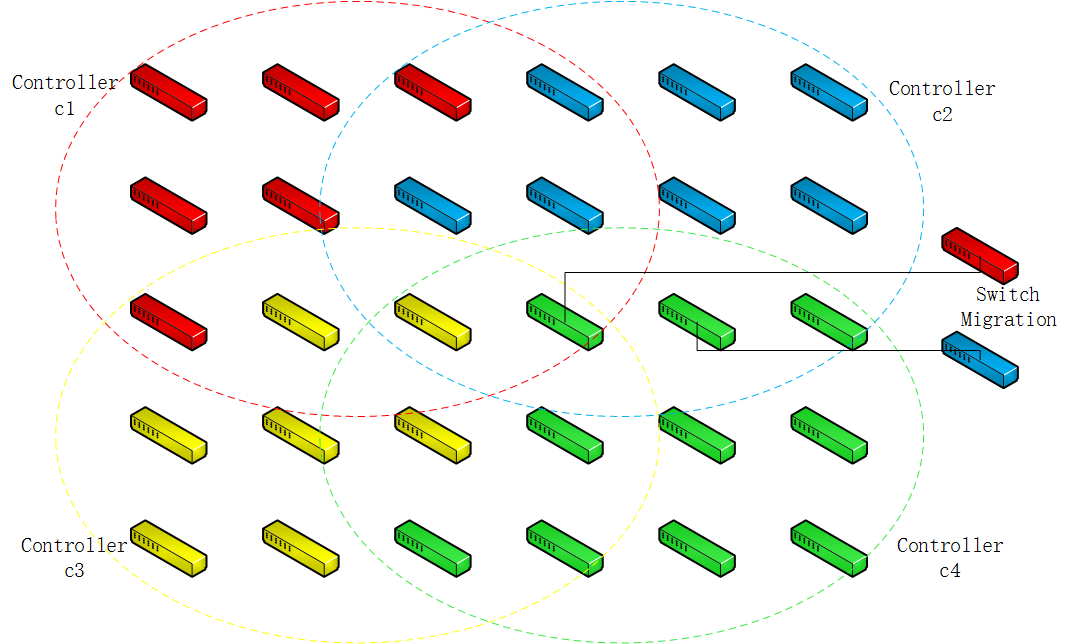
\includegraphics[scale=0.45]{chap3/before_change.png}
  \caption{An example of migrating process. There are 4 controllers in the system, Their effective areas are shown using the ellipses. The overloaded controller $c4$ manages to move the controllers to controller $c1$ and $c3$.}\label{before}
\end{figure}
\begin{figure}[htbp]
  \centering
  % Requires \usepackage{graphicx}
  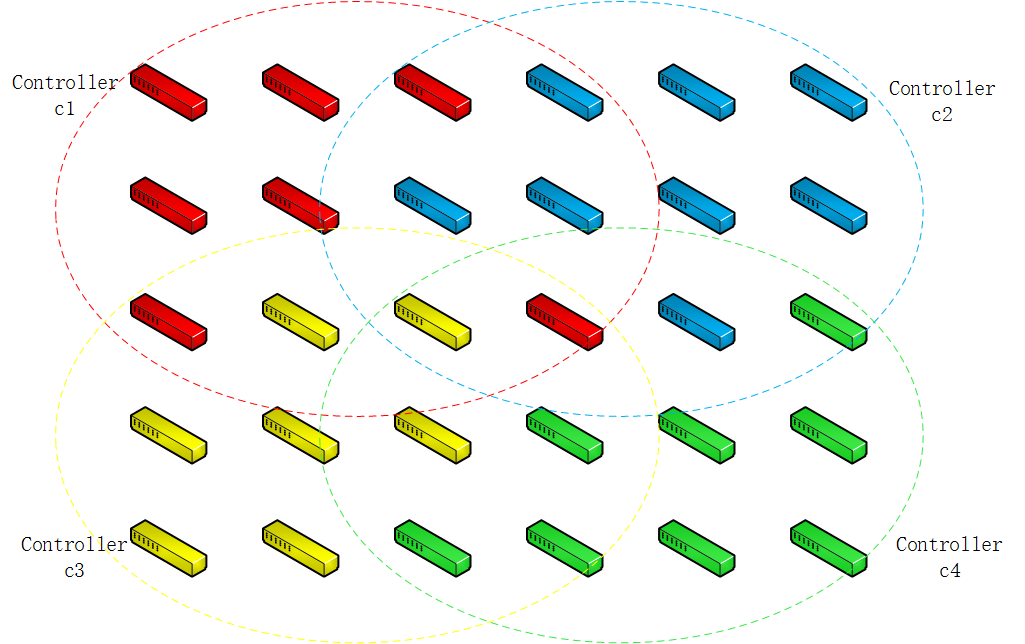
\includegraphics[scale=0.45]{chap3/after_change.png}
  \caption{The final state after the migrating process}\label{after}
\end{figure}

Actually, all the controllers can be illustrated as a connected graph for data communication. If the traffic flows vary a lot, the weight of the controller will also change because of the dynamic weight change of the switch, which leads to the result that the controller is unbalanced with other controllers. Then we must start our regional migration to migrate the switch of this controller to other available controllers to reduce the workload of the controller and keep the entire traffic balance again. The controllers can communicate between each other to ensure all the ToR-to-ToR communication can be handled. Through the above architecture, we can reduce the workload of each controller and routing component efficiently, thus can alleviate the scalability problem and the congestion problem.

We call the above statement ``naive version" because this definition is under an ideal situation. In our problem statement, we omit the performance limit of each controller. That is to say, we suppose that all the controllers in the network are the same, and has an unlimited workload capacity. In fact, in a very large data center, the distributed controllers may have very different features. For example, some of them may have a high capacity, while others have a low capacity. Let us consider the following condition: there are three controllers in the network system, say, $c_1$, $c_2$, $c_3$. The maximum capacity for $c_1$ is $\lambda$, for $c_2$ is 2$\lambda$ and for $c_3$ is 4$\lambda$. The total weight of all switches in this system is 6$\lambda$. If our naive CM-LBMC program works perfectly, then each controller will get the load of 2$\lambda$ in the end. Thus, in this condition, $c_1$ works in an overloaded status, and will definitely become the bottleneck of the system. However, $c_3$ only makes use of 50\% of its maximum abilities.

Meanwhile, we consider all the switches are equal, and all the traffic flows are equal. In Google's B4 network, they come up with the idea of high-priority traffic and low-priority traffic. This is also what we should consider in load balancing problems based on OpenFlow. If the distance between a switch and all its potential controllers are close enough, so that migrating switch $s$ from controller $c_1$ to controller $c_2$ will not influence the processing speed of messages, then we sometimes can just omit the priority of the switches. However, in some distributed data centers that has a very sparse structure, it is better to attach a switch to its nearby controllers. Meanwhile, as we have mentioned, the performance of controllers in the network system may be very different. Some of the controllers may have strong computing capacities, and thus can process messages in a higher speed. In real network systems, sometimes we hope certain messages or certain areas can have a higher priority in the whole structure, and we want to allocate switches in this region to those strong controllers.

Therefore, though for a certain switch $s_i$, it can be attached to any controller $c_j$ of its potential controller set $PC(s_i)$, the performance, or the value of the whole system may vary according to the real mapping strategy. If the value we get for $s_i$ monitored by $c_1$ is $\theta$, and for $s_i$ monitored by $c_2$ is 2$\theta$, then its better to distribute $s_i$ to $c_2$, if the current load of both controllers are below their thresholds.

Thus, in this paper we will later discuss the other two version of LBMC problem, which takes consideration of more realistic situations. But we will first establish the model of naive LBMC problem, the other versions are quite similar to this one.

We define parameter $map_{ij}=\left\{\begin{array}{ll}1 & \mbox{If } c_i \mbox{ monitors } s_j \\ 0 & \mbox{otherwise}\end{array}\right.$, Then the naive LBMC problem can be further formulated as the following linear programming:
\begin{eqnarray}
\min & \sigma=\sqrt{\frac{1}{m}\sum_{i=1}^{m} \left(\sum_{j=1}^n w(s_j)\cdot map_{ij}-\overline{w(c)}\right)^2} & \label{NLP-Object}\\
s.t. & \overline{w(c)}=\frac{1}{m}\sum_{i=1}^m \sum_{j=1}^n w(s_j)\cdot map_{ij} \label{NLP-Avg}\\
     & \sum_{i=1}^m map_{ij}=1, \quad \forall j \in [1, n] \label{NLP-Dominate} \\
     & map_{ij}=0, \quad \mbox{if } s_j \not\in RS(c_i) \mbox{ or } c_i \not\in RC(s_j), \forall i,j \label{NLP-Region}\\
     & map_{ij} \in \{0,1\} \quad \forall i, j \label{NLP-Integer}
\end{eqnarray}
Eqn.(\ref{NLP-Object}) is the standard deviation we said before. Eqn.(\ref{NLP-Avg}) calculates the average weight of all controllers. Eqn.(\ref{NLP-Dominate}) means that each switch can only have one controller as its master controller. Eqn.(\ref{NLP-Region}) means that $map_{ij}$ will be equal to 0 if controllers and switches cannot be connected logically. And Eqn.(\ref{NLP-Integer}) means $map_{ij}$ can only be an integer.

The above integer programming is proved to be NP Complete. And further adaptions to linear programming and its rounding have been discussed by predecessors, and are proved to be theoratically appliable in real conditions. Then in the next chapter, we will discuss our schemes of switch migration, and give our algorithms according to different situations.
